\section{Separately scoped trainable model-series development}
The owner authorized a bounded three-model development cycle on 10 October 2026 after the unfavorable exposed-source Combi-seq benchmark. This amendment does not replace any original numerical result, prospective architecture freeze, biological gate or confirmation requirement. It estimates retrospective aggregate expression-change prediction conditional on measured singles, a declared deposited assay and source stratum. Safe source-specific checkpoints and a common training, inference and evaluation interface are the deliverable; no universal cross-assay weights or unseen-single capability is claimed.

Opal-Base selects and fits the existing thirteen-entry reference subset inside acquired development folds, retaining observed-single additivity and a regularized correction. Opal-Interaction freezes this expert and learns a symmetric residual using a shared two-layer tanh encoder with widths 64 and 16, an elementwise latent product and an output projection. Opal-Guard learns an affine sigmoid mixture from three grouped out-of-fold expert predictions, each with its own nested selection, using graph degree, measured-single distance and source-context support. Unsupported components or sample contexts force the declared Base fallback. The mixture is not calibrated uncertainty. Missing assay, ordered genes, units or essential measured-reference inputs causes refusal.

The new configuration fixes one training seed, two penalties, Adam at learning rate 0.003, a 60-epoch branch cap and a 120-epoch gate cap with development-only stopping. The expert and gate budgets differ and are disclosed. All selections, epochs, failures and unavailable results remain saved. Final experts are shared across the variants; every variant has its own inference behavior and safe checkpoint. Held pair outcomes and unacquired labels cannot enter fitting, representation learning or inner validation. Query singles and controls are explicitly allowed.

\begin{table}[htbp]\centering
\begin{tabular}{lrrr}\toprule
Method & Combi-seq & PertSpectra TNF-positive & PertSpectra TNF-negative \\\midrule
No change & 5.713889 & 0.137007 & 0.075095 \\
Additivity & 8.993460 & 0.099904 & 0.094443 \\
Opal-Base / selected reference & 3.872700 & 0.085929 & 0.082279 \\
Historical pair-kernel family & 4.388534 & 0.085133 & 0.082056 \\
Opal-Interaction & 3.871518 & 0.086707 & 0.083545 \\
Opal-Guard & 3.871571 & 0.086159 & 0.082651 \\\bottomrule
\end{tabular}
\caption{Full-development descriptive MSE for separately fitted source-specific models. Each column uses its own reference-derived 512-gene endpoint and assay contract; absolute losses must not be pooled or compared across columns. Combi-seq equally weights 374 canonical pairs and three reported runs. Each PertSpectra context equally weights its complete pair panel and four source sample labels.}
\end{table}

The Combi-seq bank, gene endpoint, canonical outer assignments and historical predictions reproduce exactly. Interaction and Guard reduce MSE from Base by approximately 0.03\%, which does not warrant replacing Base. The original pair-kernel result remains unfavorable. Nested uniform and identity-only target-balanced prefixes use 0, 25, 50 and 100\% of available development pairs with seeds 11, 29 and 47; inner validation and cross-fitting labels count toward each budget. Outer evaluation populations remain unchanged. At zero labels only no-change and additivity are available. Pair-supervised methods are unavailable when the fixed support rules fail. The intermediate Combi-seq curves favor balanced coverage, while the nonlinear additions change error little. These are retrospective label-coverage curves, not validated active learning or prospective assay savings.

\begin{figure}[htbp]\centering
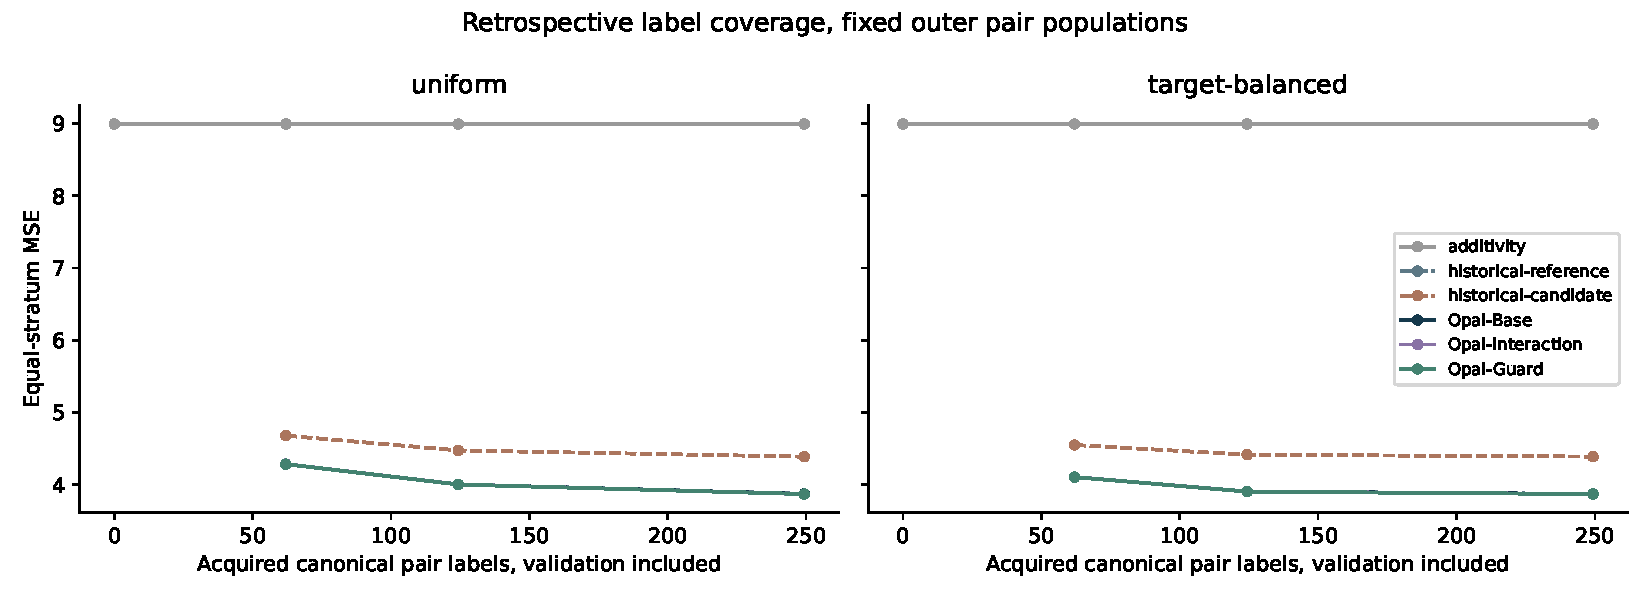
\includegraphics[width=\linewidth]{evidence/model-series-combi-learning-curves.pdf}
\caption{New series label-budget curves generated from saved records. Base and the selected historical reference overlap exactly. Every seed and budget is retained; the curves are descriptive and do not provide biological intervals.}
\end{figure}

The bounded PertSpectra extension verifies the full 3,142,132,144-byte H5AD by SHA-256 before expression decoding. Its deposited counts layer contains finite nonnegative integer values and is aggregated with bounded CSC column operations, using library-total-10000 normalization over the deposited 13,901 genes and transformation after label-conditional means. Controls have one or two control-guide calls; singles include an optional control guide. Ambiguous, intergenic and self-pair assignments are excluded. Gene labels average deposited guide mixtures and do not identify exact matched-guide causal effects. Each source sample/context retains its control, single and pair cell counts and mixtures, requiring at least ten cells and complete reference support across the four sample labels. Source preprocessing remains upstream-dependent. Reconstructing the authors' pooled condition/context count filter from metadata gives exactly the paper's 65,648 cells from 73,015 deposited rows; Opal intentionally uses a separate population and endpoint.

The resulting TNF-positive and TNF-negative panels have 108 and 52 canonical pairs, respectively. Both new nonlinear variants lose to Base in both contexts. No-change also beats every fitted model on the TNF-negative endpoint, so pair supervision is not recommended for that deposited panel. Uniform coverage is more favorable than target balancing at the observed intermediate budgets on these contexts, differing from Combi-seq. All small-budget unavailable cases, three shuffle controls and gate ablations are retained. These findings do not establish biological interaction detection, a noise ceiling, independent-culture confirmation or TNF-state transfer.

A separate leave-SampleIndex-out diagnostic trains on the other three source labels within the same TNF context while excluding every occurrence of each query pair. It uses the held sample's controls and singles, fits transforms and selects configurations within training, and weights training strata equally. Base MSE is 0.100691 in TNF-positive and 0.097187 in TNF-negative, worse than corresponding additivity errors of 0.099904 and 0.094443. Interaction and Guard use their declared Base fallback for unsupported sample contexts and therefore give identical predictions. This is transport across source sample labels, not evidence of independent cultures.

All 432 Combi-seq and 864 within-stratum PertSpectra checkpoints replay saved predictions exactly in the recorded environment. Combi-seq refits reproduce complete selection and epoch histories. Installed-wheel training, batch prediction, evaluator scoring and loading pass outside the checkout. New integrity tests join the existing Windows/Linux Python 3.11/3.14 matrix, but remote CI for these local changes is pending because the owner prohibits commits and pushes. New weights and large arrays stay local, derivative terms remain subject to release review, and the approved private GitHub v0.1.2 assets are unchanged. The independent-culture, empirical biological-power, external registration, correspondence and unapproved publication requirements remain deferred.
